% AUTHOR: ASHWIN ABRAHAM

\documentclass{beamer}
\usepackage{xcolor}
\usepackage{algpseudocode}
\usepackage{framed}
\usepackage{listings}
\usepackage{amsmath}
\usepackage{esint}
\usepackage{hyperref}
\hypersetup
{
colorlinks=true,
linkcolor=blue,
filecolor=magenta,      
urlcolor=cyan,
pdftitle={Parameterized verification through view abstraction},
pdfpagemode=FullScreen,
}
\usepackage[utf8]{inputenc}

\usetheme{Madrid}
\usecolortheme{default}


\title[] 
{Presentation:\\Linear Invariant Generation Using Non-Linear Constraint Solving}


\author[Ashwin Abraham] 
{Ashwin Abraham}

\institute[IIT-B] 
{
    IIT Bombay
}

\date[2023]
{26th September, 2023}

% \logo{\includegraphics[height=2cm]{iitb-logo.png}}


\begin{document}
    \frame{\titlepage}

    \begin{frame}
        \frametitle{Table of Contents}
        \tableofcontents    
    \end{frame}

    \section{Abstract}
    {
        \begin{frame}
            \frametitle{Abstract}
            A method is presented for generating linear invariants for transition systems that reduces to a non-linear constraint solving problem. 
        \end{frame}
    }

    \section{Preliminaries}
    {
        \begin{frame}{Transition System}
            A transition system $P$ is a tuple $\langle V, L, l_{0}, \Theta, \mathcal{T} \rangle$ where $V$ is a set of variables, $L$ is a set of locations, $l_{0} \in L$ is an initial location, $\Theta$ is an initial assertion over the variables $V$, and $\mathcal{T}$ is a set of transitions of the form $(l, l', \rho_{\tau})$, where $\rho_{\tau}$ is an assertion over $V \cup V'$ that serves as the transition condition. We use $V'$ to distinguish the variables pre and post transition. It is not the case that each location has it's own variable set, but rather that for transitions, we would like to have constraints relating the values of the variables before and after the update. We assume that $V = \{x_{1}, \dots x_{n}\}$ throughout the paper. For any formula $\psi$ over variables $V$, we denote the formula obtained by replacing the variables in $V$ with the corresponding variables in $V'$ by $\psi'$.
        \end{frame}
        \begin{frame}{Transition System}
            \begin{figure}[h!]
                \includegraphics[scale=0.7]{transition_system.png}
            \end{figure}
            \begin{center}
                Draw CFG for this system [on whiteboard]
            \end{center}
        \end{frame}
        \begin{frame}{Control Flow Graph}
            The CFG of a transition system is a graph whose vertices are the locations of the transition system and whose edges are the transitions between the locations and are labelled by the transition condition. For a path $\pi$ in the CFG, the conjunction of the transition conditions of each edge in the graph is called the transition condition for the path, $\rho_{\pi}$.

            A \textbf{cutset} of a transition system is a subset of locations such that every cycle in the CFG passes through the subset. A location in a cutset is called a \textbf{cutpoint}. A \textbf{basic path} is a path from one cut point to another that does not pass through any other cut points. Any cycle can be broken up into a sequence of basic paths.
        \end{frame}
        \begin{frame}{Inductive Assertion Maps}
            Given a transition system $P$ with a cutset $C$. A mapping $\eta : C \rightarrow Assertions$ is called an inductive assertion map iff for all cutpoint $l,  l' \in C$ the following hold:
            \begin{enumerate}
                \item For each basic path $\pi$ from $l_{0}$ to $l$, $\Theta \land \rho_{\pi} \implies \eta(l)$ (Initialization)
                \item For each basic path $\pi$ from $l$ to $l'$, $\eta(l) \land \rho_{\pi} \implies \eta(l')$ (Consecution)
            \end{enumerate}
            % If we are given a post-image operator
            A $k$-linear inductive assertion map is one where each $\eta(l)$ is $k$-linear (See the next slide for the definition of $k$-linearity).
        \end{frame}
        \begin{frame}{Linear and Non-Linear Constraints}
            % \vspace*{-5mm}
            \begin{itemize}
                \item A linear constraint over $V$ is an inequality of the form $\sum\limits_{i = 1}^{n} a_{i}x_{i} + b \leq 0$
                \item If $b = 0$, we call it a homogenous constraint
                \item A linear assertion over $V$ is a conjunction of linear constraints
                \item An assertion consisting of $k$ clauses is said to be $k$-linear
                \item Linear assertions correspond to polyhedra in $\mathbb{R}^n$
                \item Given a set of vectors $S$, $cone(S)$ is the set of finite positive linear combinations of vectors in $S$. A cone is said to be \textit{finitely generated} if there exists a finite subset $S'$ of $S$ such that $cone(S') = cone(S)$. A fundamental result states that a cone is finitely generated iff it is a polyhedron
                \item A non linear constraint over $V$ is an inequality of the form $P(x_{1}, \dots x_{n}) \leq 0$, where $P$ is a polynomial. A non-linear assertion is a conjunction of such constraints. The solution set of a non-linear assertion is called a semi-algebraic set.
                \item We say a transition system $P$ is linear iff $\Theta$ and $\rho_{\tau}$ are linear assertions. We deal only with linear transition systems.
            \end{itemize}
        \end{frame}
        \begin{frame}{Farkas' Lemma}
            Let $S$ be an $m$-linear assertion over variables $\{x_{1}, \dots x_{n}\}$ of the form
            \begin{equation*}
                \sum\limits_{j = 1}^{n} a_{ij}x_{j} + b_{i} \leq 0, i \in \{1, \dots m\}
            \end{equation*}
            If $S$ is satisfiable and $\psi$ is some linear constraint of the form
            \begin{equation*}
                \sum\limits_{j = 1}^{n}c_{j}x_{j} + d \leq 0
            \end{equation*}
            Then we have $S \implies \psi$ if and only if there exist non-negative $\lambda_{0}, \lambda_{1}, \dots \lambda_{m}$ such that
            \begin{equation*}
                \psi \equiv -\lambda_{0} + \sum\limits_{i = 1}^{m} \lambda_{i} S_{i} \leq 0
            \end{equation*}
            where $S_{i}$ is $\sum\limits_{j = 1}^{n} a_{ij}x _{j} + b$. Furthermore, $S$ is unsatisfiable if and only if the inequality $1 \leq 0$ can be obtained this way.
        \end{frame}
        \begin{frame}{Farkas' Lemma}
            We use a tabular format to represent applications of Farkas' Lemma.
            \begin{figure}[h!]
                \includegraphics[scale=0.8]{farkas.png}
            \end{figure}
            The antecedents are placed above the line and the consequences below. For each column, the sum of the column entries above the line, with the appropriate multipliers, must be equal to the entry below the line. If a row corresponds to an inequality, the corresponding multiplier is required to be non-negative. This requirement is dropped for rows corresponding to equalities.
        \end{frame}
    }
    \section{Generating Invariants}
    {
        \begin{frame}{Generating Invariants}
            The approach to generating invariants is based on Farkas' Lemma. Given a transition system $P$, we write down the initiation and consecution conditions for each cutpoint $l$, and apply Farkas' Lemma on the conditions to generate the constraints. We parametrize each clause of each inductive assertion by the coefficients of the clause. We end up applying Farkas' Lemma on all basic paths from $l_{0}$ to $l$, on all basic paths from $l$ to $l'$, where $l$ and $l'$ are cutpoints, and for each clause of $\eta(l)$ and $\eta(l')$.

            The condition that Farkas' Lemma gives us is a disjunction, corresponding to 2 possibilities - either the system is satisfiable or it is not. Paths for which the system is not satisfiable are known as disabled paths, and those for which it is are known as enabled paths. Therefore at the end, we get an existentially quantified CNF formula where each clause is a disjunction of two assertions. 

            If there are $a$ initialization paths and $b$ consecution paths, the number of clauses we get would be $ak + bk^2$. It is found that for $k > 1$, solving this becomes too computationally intensive, except for the simplest systems.
        \end{frame}
        \begin{frame}{Generating Invariants}
            \begin{figure}[h!]
                \includegraphics[scale=0.7]{transition_system.png}
            \end{figure}
            \begin{center}
                Generate invariants for this system [on whiteboard]
            \end{center}
        \end{frame}
        \begin{frame}{Soundness and Completeness}
            The solutions generated by our method correspond precisely to the set of $k$-linear inductive assertion maps, ie our method is both sound and complete. This follows as Farkas' Lemma is sound and complete.
        \end{frame}
    }

    \section{Solving Non-Linear Constraints}
    {
        \begin{frame}{Solving Non-Linear Constraints}
            Non-Linear constraints are generated by the enabled consecution paths, as for an enabled basic path from $\eta(l)$ to $\eta(l')$, we will be multiplying the (unknown) coefficients of $\eta(l)$ by another unknown.

            The Linear constraints can be solved by techniques such as Fourier-Motzkin elimination. For Non-Linear constraints, the method used is \textit{Cylindrical Algebraic Decomposition}, introduced by Collins. Another approach is to use Linear Programming and delay solving non-linear constraints until they can be linearized or at least simplified. 

            Many heuristics have also been developed to simplify solving these constraints.

            A tool known as \texttt{REDLOG}, that incorporates many of these techniques and heuristics, has been used to compute the solutions.
        \end{frame}
    }

    % \section{Interprocess communication}
    % {
    %     \begin{frame}
    %         \frametitle{The Topology of a system}
    %         \begin{itemize}
    %             \item The topology of a system refers to which processes can communicate with (ie inspect the state of) other processes.
                
    %             \item Some common topologies are:
    %             \begin{enumerate}
    %                 \item Linear Topology:\\Here the processes are ordered in an array and each process can distinguish the states to its left and those to its right. It can inspect the state of any of these processes.
    %                 \item Ring Topology:\\The processes are ordered in a ring, and each process can only inspect the state of the process next to it.
    %                 \item Tree Topology:\\The processes are arranged in a tree and each process can distinguish its parent process and child processes and inspect their states.
    %                 \item Multiset Topology:\\Each process can distinguish every other process and inspect their states.
    %             \end{enumerate}
    %         \end{itemize}
    %     \end{frame}

    %     \begin{frame}
    %         \frametitle{The Topology of a system}
    %         We can represent the topology of a system by a directed graph $G(V, E)$ where the vertices correspond to processes, and there is an edge from 
    %         vertex $A$ to vertex $B$ if process $A$ can inspect the state of process $B$.
    %         % \begin{figure}
    %         %     \begin{center}
    %         %         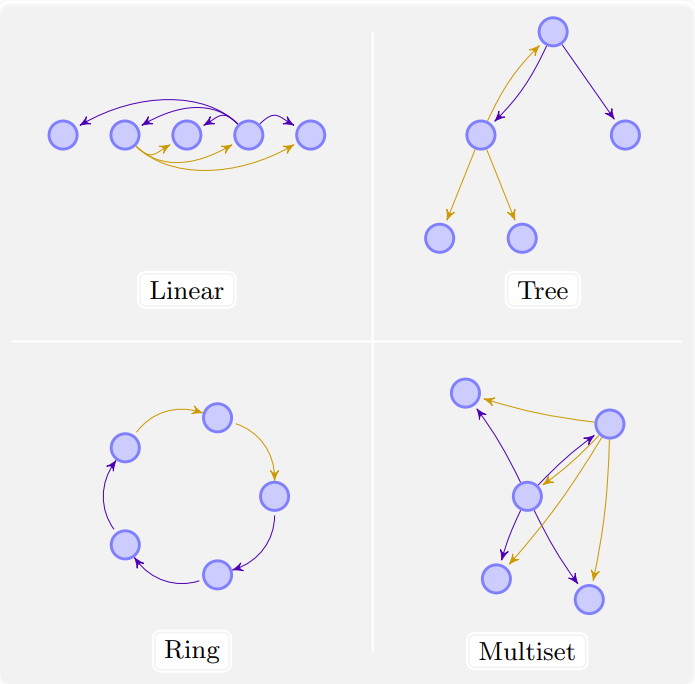
\includegraphics[scale=0.4]{images/topologies.png}
    %         %         \caption{The graphs of the above mentioned topologies}
    %         %     \end{center}
    %         % \end{figure}
    %     \end{frame}

    %     \begin{frame}
    %         \frametitle{Local and Global Transitions}
    %         \begin{itemize}
    %             \item If a process transitions from one state to another without needing to inspect the states of other processes, the transition is known as a local transition.
    %             \item On the other hand, if the transition is dependent on the states of other processes, the transition is called a global transition.
    %             \item A major issue that arises is that global transitions are not checked atomically. The state of an inspected process may change while other processes are still being inspected.
    %             \item The method presented provides an elegant solution to this issue.
    %         \end{itemize}
    %     \end{frame}

    %     \begin{frame}
    %         \frametitle{Other Transitions}
    %         \begin{itemize}
    %             \item Broadcast Transitions: Here, an arbitrary number of processes change their state simultaneously. 
    %             A broadcast transition has an initiator that causes a (possibly empty) subset of the processes that can inspect its state to transition.
    %             \item Rendezvous Transitions: Here a fixed number of processes change their state simultaneously. 
    %             \item Shared Variable Update: Here, the shared variable is a part of the state of multiple processes, and when it is updated by any of the 
    %             processes, the other processes change their state to reflect the updated value of the variable.
    %             \item Process Creation and Deletion make the topology of our system dynamic, but these can be reframed in terms of rendezvous transitions, as we 
    %             will see later.
    %         \end{itemize}
    %     \end{frame}
    % }

    % \section{Formalism}
    % {
    %     \begin{frame}
    %         \frametitle{Formalism}
    %         To simplify our results, for now we will work with parametrized systems having identical processes and a linear topology, and that all transitions are either local or global. We assume for now that global checks are atomic, although we will soon drop this condition. We also assume that each process is governed by a finite state automaton.
    %         \begin{itemize}
    %             \item For a given topology, a parametrized system can be defined as the pair $\mathcal{P} = (\mathcal{Q}, \Delta)$, where $\mathcal{Q}$ is the set of \textit{local states} of each process and $\Delta$ is a set of transition rules over processes.
    %             \item A local transition rule will be of the form $s_{i} \rightarrow s'_{i}$, where $s_{i}, s'_{i} \in \mathcal{Q}$ refer to the states of the $i^{th}$ process before and after transition.
    %             \item A global rule is of the form $Q  j \sim i : s_{j} \in S \implies s_{i} \rightarrow s'_{i}$. Here $Q$ is a quantifier (either $\forall$ or $\exists$) and $\sim$ is some relation dependent on the topology of the system (for a linear topology it can be either $<$, $>$ or $\neq$)
    %             and $S$ is some subset of $\mathcal{Q}$.
    %         \end{itemize}
    %     \end{frame}

    %     \begin{frame}
    %         \frametitle{Formalism}
    %         \begin{itemize}
    %             \item The configuration $c$ of the system is a word over the alphabet $\mathcal{Q}$, ie, an array of states. We denote the set of all configurations as $\mathcal{C}$.
    %             \item $\left|c\right|$ denotes the number of processes. This is the parameter with which we parametrize the system.
    %             \item $c_{i}$ denotes the state of the $i^{th}$ process in configuration $c$, for $1 \leq i \leq \left|c\right|$.
    %             \item For a local rule $\delta \in \Delta$ such that $\delta = a \rightarrow b$, we say $c' = \delta(c, i)$ if $c'$ is the result of applying $\delta$ on the $i^{th}$ process.
    %             In particular, for $\delta(c, i)$ to be defined, $c_{i}$ must be $a$, and $\delta(c, i)_{i}$ will be $b$.
    %             \item For a global rule $\delta \in \Delta$ such that $\delta = Q j \sim i: s_{j} \in S \implies a \rightarrow b$, $\delta(c, i)$ is defined iff $c_{i} = a$, and the condition $Q j \sim i: s_{j} \in S$ is satisfied. In this case, $\delta(c, i)_{i} = b$.
    %             \item We write $c \xrightarrow[]{\delta} c'$ if $c' = \delta(c, i)$ for some $i \in \{1 \dots c\}$, and we define $\xrightarrow[]{*}$ as the reflexive and transitive closure of $\xrightarrow[]{\delta}$ (possibly with different $\delta$s).
    %         \end{itemize}
    %     \end{frame}

    %     \begin{frame}
    %         \frametitle{Reachability}
    %         \begin{itemize}
    %             \item We say that a configuration $c'$ is reachable from $c$ if $c \xrightarrow[]{*} c'$.
    %             \item The \textit{reachability problem} is defined by a parametrized system $\mathcal{P} = (\mathcal{Q}, \Delta)$, a set of initial states $\mathcal{I} \subseteq \mathcal{C}(\mathcal{P})$ and a set of bad states $\mathcal{B} \subseteq \mathcal{C}(\mathcal{P})$. 
    %             \item We define the set $\mathcal{R}$ of reachable states as $\{c \in C: \exists c' \in \mathcal{I}, c' \xrightarrow[]{*} c\}$. We say a $\mathcal{P}$ is \textit{safe} with respect to $\mathcal{I}$, $\mathcal{B}$ iff $\mathcal{R} \cap \mathcal{B} = \emptyset$.
    %             \item In order to define the \textit{bad} set $\mathcal{B}$ independently of the parameter, we define it as the closure of a set of minimal bad configurations, ie $\mathcal{B} = \{c \in \mathcal{C}: \exists b \in \mathcal{B}_{min}: b \sqsubseteq c\}$, where $\sqsubseteq$ denotes 
    %             a relation (known as the \textit{covering} relation) dependent on the topology of the system (for a linear topology it'll be the subword relation).
    %             \item $\mathcal{I}$ and $\mathcal{R}$ are also defined independently of the parameter this way.
    %             \item $\mathcal{S}_{k}$ denotes $\{c \in S: \left|c\right| = k\}$ for $S = \mathcal{I}$, $\mathcal{B}$, $\mathcal{R}, \mathcal{C}$. 
    %         \end{itemize}
    %     \end{frame}
    % }
    % \section{Szymanski's Protocol}
    % {
    %     \begin{frame}
    %         \frametitle{Szymanski's Protocol}
    %         \begin{itemize}
    %             \item Szymanski's Protocol is a protocol that is used to ensure mutually exclusive access to a resource for a finite number of processes.
    %             \item It is based on the analogy of a waiting room with an entry door and an exit door that gives access to the resource.
    %             \item Each process has a flag with $5$ possible values:
    %             \begin{itemize}
    %                 \item \textbf{0}: The process declares that it doesn't want to access the resource right now (it is outside the waiting room)
    %                 \item \textbf{1}: The process declares that it wants to enter the critical section, and it is outside the waiting room.
    %                 \item \textbf{2}: The process is waiting for other processes to enter the waiting room.
    %                 \item \textbf{3}: The process has just entered the waiting room.
    %                 \item \textbf{4}: The process is about to start or in the critical section.
    %             \end{itemize}
    %             \item The flag of a process can be read by every other process but can be changed only by itself.
    %         \end{itemize}            
    %     \end{frame}

    %     \begin{frame}
    %         \frametitle{Szymanski's Protocol}
    %         \begin{itemize}
    %             \item In the beginning, all the processes that request entry at roughly the same time, enter the waiting room one by one. 
    %             \item The last of these closes the entry door and waits for the processes of lower IDs to leave the waiting room and finish accessing the resources.
    %             \item Once the lower ID processes are done, they change their flags to \textbf{0} or \textbf{1} to indicate this. The last process finishing resource access causes the entry door to be opened.
    %             \item For now, we assume that all these checks can be done atomically.
    %         \end{itemize}
    %     \end{frame}

    %     \begin{frame}[fragile]
    %         \frametitle{Szymanski's Protocol}
    %         The pseudocode for this protocol is as follows:
    %         % \begin{figure}
    %         %     \begin{center}
    %         %         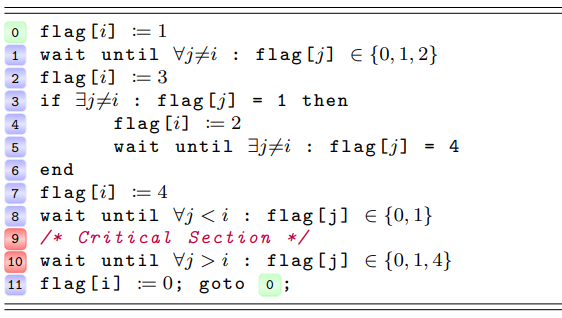
\includegraphics[scale=1]{images/codeimg.png}
    %         %         % \caption{}
    %         %     \end{center}
    %         % \end{figure}
    %     \end{frame}

    %     \begin{frame}
    %         \frametitle{Szymanski's Protocol}
    %         \begin{itemize}
    %             \item The configuration of the system here is a word over the alphabet $\{0, 1, \cdots 11\}$.
    %             \item The initial configuration of the system has all processes in state $0$.
    %             \item $\mathcal{I} = \{0, 0.0, 0.0.0 \cdots\}$
    %             \item The bad configurations are those where more than one process is in state $9$ or state $10$.
    %             \item $\mathcal{B} = \{9.9, 9.10, 10.9, 10.10, \cdots\}$
    %         \end{itemize}
    %     \end{frame}
    % }
    % \section{View Abstraction}
    % {
    %     \begin{frame}
    %         \frametitle{Verification}
    %         \begin{itemize}
    %             \item The key insight here is that small instances of the system give enough information to predict the behaviour for all values of 
    %             the parameter.
    %             \item On a high level, we can say that this occurs because the patterns that occur for lower values of the parameter repeat themselves for larger values.
    %             \item The configurations for higher parameters cover those of lower parameters, in a sense.
    %             \item Our algorithm automatically detects a cutoff point $n$ such that we only need to compute $\mathcal{R}_{1}, \mathcal{R}_{2} \cdots \mathcal{R}_{n}$ to determine whether $\mathcal{R} \cap \mathcal{B} = \emptyset$. 
    %             \item To do this, we perform \textit{overapproximation}, where we abstract the system such that $\mathcal{R} \subseteq R'$. Now if we are able to show $\mathcal{R}' \cap B = \emptyset$, we can conclude that $\mathcal{R} \cap B = \emptyset$.
    %         \end{itemize}
    %     \end{frame}

    %     \begin{frame}
    %         \frametitle{View Abstraction}
    %         \begin{itemize}
    %             \item We first focus only on \textit{atomically} checked global conditions. As mentioned earlier, we will remove this restriction soon.
    %             \item In \textit{view abstraction}, we consider the configurations from the perspective of a few \textit{fixed} number of processes. This abstraction is parametrized by $k$, the number of processes.
    %             \item The new construct made by considering the perspective of only the $k$ processes taken is called a \textit{view}.
    %             \item We have a certain freedom in choosing what information to discard and what to retain while constructing the view.
    %             \item For example, a simple example of a view would be a subword of the configuration $c$, with size $k$.
    %         \end{itemize}
    %     \end{frame}

    %     \begin{frame}
    %         \frametitle{The Subword View}
    %         \begin{itemize}
    %             \item Here, a view of a configuration $c$ with size $k$ is a subword of $c$ with size $k$.
    %             \item We denote the set of views by $\mathcal{V}$ and the set of views of size \textit{upto} $k$ by $\mathcal{V}_{k}$. Note that a view is also a valid configuration, and therefore $\mathcal{V}_{k} \subseteq \mathcal{C}$.
    %             \item We now define two functions:
    %             \begin{enumerate}
    %                 \item The \textit{abstraction} function $\alpha_{k}: \mathcal{C} \rightarrow 2^{\mathcal{V}_{k}}$ that maps a configuration to the set of all it's subwords of size at most $k$.
    %                 \begin{equation*}
    %                     \alpha_{k}(c) = \{v \in \mathcal{V}_{k}: v \sqsubseteq c\}, \forall c \in \mathcal{C}
    %                 \end{equation*}
    %                 \item We also define the \textit{abstraction} for subsets of $\mathcal{C}$ as $\alpha_{k}: 2^{\mathcal{C}} \rightarrow 2^{\mathcal{V}_{k}}$ as
    %                 \begin{equation*}
    %                     \alpha_{k}(S) = \{v \in \mathcal{V}_{k}: \exists c \in S: v \sqsubseteq c\} = \bigcup\limits_{c \in S} \alpha_{k}(c), \forall S \subseteq \mathcal{C}
    %                 \end{equation*}
    %                 \item The \textit{concretization} function $\gamma_{k}: 2^{\mathcal{V}_{k}} \rightarrow 2^\mathcal{C}$ that maps a set of views to the set of configurations that can be reconstructed from those views, ie
    %                 \begin{equation*}
    %                     \gamma_{k}(V) = \{c \in \mathcal{C}: \alpha_{k}(c) \subseteq V\}, \forall V \subseteq \mathcal{V}_{k}
    %                 \end{equation*}
    %             \end{enumerate}
    %         \end{itemize}
    %     \end{frame}

    %     \begin{frame}
    %         \frametitle{Galois Connection (Lemma 1)}
    %         \begin{itemize}
    %             \item We can order $2^{\mathcal{C}}$ and $2^{\mathcal{V}_{k}}$ by defining $x \leq y$ when $x \subseteq y$, $\forall x, y \in 2^{\mathcal{C}}$ or $\forall x, y \in 2^{\mathcal{V}_{k}}$.
    %             \item With this ordering, $\alpha_{k}$ and $\gamma_{k}$ become monotonic functions.
    %             \item $\forall V \subseteq \mathcal{V}_{k}, \alpha_{k}(\gamma_{k}(V)) \subseteq V$. This is because $\forall c \in \gamma_{k}(V)$, $\alpha_{k}(c) \subseteq V$ (by the definition of $\gamma_{k}$).
    %             \item $\forall S \subseteq C, S \subseteq \gamma_{k}(\alpha_{k}(S))$. This is because $c \in S \implies \alpha_{k}(c) \subseteq \alpha_{k}(S)$ (by monotonicity), which implies that $c \in \gamma_{k}(\alpha_{k}(S))$.
    %         \end{itemize}
    %         If $(A, \leq)$ and $(B, \leq)$ are two posets, we say two monotone functions $F: A \rightarrow B$ and $G: B \rightarrow A$ form a Galois Connection iff
    %         \begin{equation*}
    %             \forall a \in A, \forall b \in B, F(a) \leq b \Leftrightarrow a \leq G(b)
    %         \end{equation*}
    %         Now, $\alpha_{k}(A) \subseteq B \implies \gamma_{k}(\alpha_{k}(A)) \subseteq \gamma_{k}(B) \implies A \subseteq \gamma_{k}(B)$. Similiarly, we can prove the converse. Therefore, $\alpha_{k}$ and $\gamma_{k}$ form a Galois connection.
    %     \end{frame}

    %     \begin{frame}
    %         \frametitle{Monotonicity of $\gamma_{k}\alpha_{k}$ (Lemma 2)}
    %         Lemma:
    %         \begin{equation*}
    %             \forall X \subseteq \mathcal{C}, X \subseteq \cdots \gamma_{2}(\alpha_{2}(X)) \subseteq \gamma_{1}(\alpha_{1}(X))
    %         \end{equation*}
    %         Proof:\\
    %         Since $\alpha_{k}(S) \subseteq \alpha_{k + 1}(S)$, we define $f_{k + 1}(S)$ as $\alpha_{k + 1}(S) - \alpha_{k}(S)$.
    %         Now, $\gamma_{k + 1}(\alpha_{k + 1}(X)) = \{c \in C: \alpha_{k + 1}(c) \subseteq \alpha_{k + 1}(X)\} = \{c \in C: \alpha_{k}(c) \cup f_{k + 1}(c) \subseteq \alpha_{k}(X) \cup f_{k + 1}(X)\}$.
    %         Since $\forall M, N, f_{k+1}(M) \cap \alpha_{k}(N) = \emptyset$, this is possible only when $\alpha_{k}(c) \subseteq \alpha_{k}(S)$ and $f_{k+1}(c) \subseteq f_{k + 1}(S)$, ie 
    %         \begin{equation*}
    %             \gamma_{k + 1}(\alpha_{k + 1}(S)) = \{c \in \mathcal{C}: \alpha_{k}(c) \subseteq \alpha_{k}(S) \land f_{k + 1}(c) \subseteq f_{k + 1}(S)\}
    %         \end{equation*}
    %         Therefore, 
    %         \begin{equation*}
    %             \gamma_{k + 1}(\alpha_{k + 1}(S)) \subseteq \{c \in \mathcal{C}: \alpha_{k}(c) \subseteq \alpha_{k}(S)\} = \gamma_{k}(\alpha_{k}(S))
    %         \end{equation*}
    %         This means that, although $\gamma_{k}(\alpha_{k}(S))$ is an overapproximation of $S$, as we increase the value of $k$, it becomes a better overapproximation. 
    %     \end{frame}

    %     \begin{frame}
    %         \frametitle{Some more terminology}
    %         If we find a $k$ such that $\mathcal{B} \cap \gamma_{k}(\alpha_{k}(\mathcal{R})) = \emptyset$, then we can conclude that $\mathcal{B} \cap \mathcal{R} = \emptyset$. This is the gist of our algorithm.\\
    %         Some more terminology:
    %         \begin{itemize}
    %             \item For a set of configurations $X \subseteq \mathcal{C}$, we define its \textit{post-image} $post(X)$ as the set $\{\delta(c, i) | c \in X, i \leq |c|, \delta \in \Delta\}$.
    %             \item We also define $post^{*}(X) = \{c \in \mathcal{C} : \exists c' \in X : c' \xrightarrow[]{*} c \}$. Since we deal only with transitions that do not change the topology of the system, $\mathcal{R}_{k} = post^{*}(\mathcal{I}_{k})$.
    %             \item We define the \textit{abstract post-image} of a set of views $V \subseteq \mathcal{V}_{k}$ as $\alpha_{k}(post(\gamma_{k}(V)))$. This represents the set of views that may be obtained after one transition of the system.
    %         \end{itemize}
    %     \end{frame}
    % }

    % \section{The Algorithm and its Implementation}
    % {
    %     \begin{frame}
    %         \frametitle{The Algorithm}
    %         \begin{itemize}
    %             \item The algorithm determines a cutoff point $K$ such that a set of views $V \subseteq \mathcal{V}_{K}$ computed by the algorithm satisfy
    %             \begin{enumerate}
    %                 \item $\alpha_{K}(\mathcal{I}) \subseteq V$, $Apost_{K}(V) \subseteq V$ and $\mathcal{R} \subseteq \gamma_{K}(V)$
    %                 \item $\gamma_{K}(V) \cap \mathcal{B} = \emptyset$
    %             \end{enumerate}
    %             \item If we can find such a $V$, then we can conclude that $\mathcal{R} \cap \mathcal{B} = \emptyset$.
    %             \item We iterate through the values of $k \in \mathbb{N}$ to find such a $V \subseteq \mathcal{V}_{k}$.
    %             \item For each value of $k$, we first check that $\mathcal{R}_{k} \cap \mathcal{B} = \emptyset$. If this is not the case, we can stop and say that the system is unsafe.
    %             \item We then proceed to calculate a fixed point $V$ of $\cup Apost_{k}$ that contains $\alpha_{k}(\mathcal{I})$, ie $V \subseteq \mathcal{V}_{k}$ such that $\alpha_{k}(\mathcal{I}) \subseteq V$ and $Apost_{k}(V) \subseteq V$.
    %             \item It can be shown that if $\alpha_{k}(\mathcal{I}) \subseteq V$ and $Apost_{k}(V) \subseteq V$, then $\mathcal{R} \subseteq \gamma_{k}(V)$. Therefore, this $V$ satisfies the first condition of our algorithm.
    %             \item We thus just have to check whether $\gamma_{k}(V) \cap \mathcal{B} = \emptyset$. If this is the case, we can conclude that the system is safe, and if not, we proceed to the next value of $k$.
    %         \end{itemize}
    %     \end{frame}

    %     \begin{frame}
    %         \frametitle{Lemma 3}
    %         Lemma: If $\alpha_{k}(\mathcal{I}) \subseteq V$ and $Apost_{k}(V) \subseteq V$, then $\mathcal{R} \subseteq \gamma_{k}(V)$\\
    %         Proof:\\
    %         If $\alpha_{k}(\mathcal{I}) \subseteq V$, then since $\alpha_{k}$ and $\gamma_{k}$ form a Galois connection, $\mathcal{I} \subseteq \gamma_{k}(V)$.
    %         Similiarly, $Apost_{k}(V) = \alpha_{k}(post(\gamma_{k}(V))) \subseteq V \implies post(\gamma_{k}(V)) \subseteq \gamma_{k}(V)$. Therefore, $\gamma_{k}(V)$ contains $\mathcal{I}$ 
    %         and is a fixed point of $\cup post$. Therefore, by iteration, $\mathcal{R} = post^{*}(\mathcal{I}) \subseteq \gamma_{k}(V)$.
    %     \end{frame}

    %     \begin{frame}
    %         \frametitle{The Implementation}
    %         \begin{itemize}
    %             \item In order to implement the first step of the algorithm, we will need to calculate $\mathcal{R}_{k} = post^{*}(\mathcal{I}_{k})$.
    %             \item This can be done quite easily, by repeatedly applying $\cup post$ on $\mathcal{I}_{k}$ until a fixed point is reached. Since $\mathcal{R}_{k}$ is finite, this will terminate eventually.
    %             \item For the second step of the algorithm, we first set $V = \alpha_{k}(\mathcal{I})$. $\mathcal{I}$ is usually a regular set, and therefore we can construct an automaton accepting only subwords of $\mathcal{I}$ of size atmost $k$. $\alpha_{k}(\mathcal{I})$ is then the set of words in $\mathcal{V}_{k}$ accepted by this automaton. 
    %             \item We then repeatedly apply $V \leftarrow V \cup Apost_{k}(V)$ until a fixed point is obtained. Since $V \subseteq \mathcal{V}_{k}$ which is a finite set, a fixed point will always be obtained after a finite number of iterations.
    %             \item The only problem is in computing $Apost_{k}(V)$, as $\gamma_{k}(V)$ can be infinite. We bypass this problem by computing only $\gamma_{k}(V) \cap \mathcal{V}_{k + 1}$. We show that this is sufficient 
    %             to compute $\cup Apost_{k}$.
    %         \end{itemize}
    %     \end{frame}

    %     \begin{frame}
    %         \frametitle{Lemma 4}
    %             Formally, for $\ell \geq 0$ and $V \subseteq \mathcal{V}_{k}$, we define 
    %             \begin{equation*}
    %                 \oint\limits_{k}^{\ell} V = \{c \in \mathcal{C} : \alpha_{k}(c) \subseteq V \wedge \left|c\right| \leq \ell\}
    %             \end{equation*}
    %             Lemma: For any $V \subseteq \mathcal{V}_{k}$,
    %             \begin{equation*}
    %                 V \cup Apost_{k}(V) = V \cup \alpha_{k}(post(\oint\limits_{k}^{k + 1}V))
    %             \end{equation*}
    %     \end{frame}

    %     \begin{frame}{Proof of Lemma 4}
    %         Some terminology - for a configuration $c \in \mathcal{C}$ and a set $\mathbb{P} = \{i_{1}\cdots i_{k}\} \subseteq \{1\cdots \left|c\right|\}$, denote the view $c_{i_{1}}\cdots c_{i_{k}}$ as $view(c, \mathbb{P})$.

    %         Two observations:
    %         \begin{enumerate}
    %             % \item $\forall c_{1}, c_{2} \in \mathcal{C}$ and for all sets $\mathbb{P}$ and transitions $\delta \in \Delta$, $view(c_{1}, \mathbb{P}) \xrightarrow[]{\delta} view(c_{2}, \mathbb{P}) \implies c_{1} \xrightarrow[]{\delta} c_{2}$.
    %             \item If $\delta \in \Delta$ is a local transition or a universally quantified transition, $\forall c_{1}, c_{2} \in \mathcal{C}$, if $c_{1} \xrightarrow[]{\delta} c_{2}$, then for all sets $\mathbb{P}$, either $view(c_{1}, \mathbb{P}) = view(c_{2}, \mathbb{P})$ or $view(c_{1}, \mathbb{P}) \xrightarrow[]{\delta} view(c_{2}, \mathbb{P})$.
    %             \item If $\delta \in \Delta$ is an existentially quantified transition, say of the form $\exists j \sim i : s_{j} \in S \implies s_{i} \rightarrow s'_{i}$ and $c_{1} \xrightarrow[]{\delta} c_{2}$, then if the set $\mathbb{P}$ contains both $i$ and $j$ (ie both the transitioning state and the witness), then $view(c_{1}, \mathbb{P}) \xrightarrow[]{\delta} view(c_{2}, \mathbb{P})$. 
                
    %             If $i \notin \mathbb{P}$, then clearly $view(c_{1}, \mathbb{P}) = view(c_{2}, \mathbb{P})$.
    %         \end{enumerate}
    %     \end{frame}

    %     \begin{frame}{Proof of Lemma 4}
    %         Now, by definition, $\oint\limits_{k}^{k + 1} V \subseteq \gamma_{k}(V)$, and therefore $V \cup \alpha_{k}(post(\oint\limits_{k}^{k + 1} V)) \subseteq V \cup Apost_{k}(V)$. %To prove the lemma we %just have to show that $\forall v \in Apost_{k}(V) - V, v \in \alpha_{k}(post(\oint\limits_{k}^{k + 1} V))$, ie $\exists c \in post(\oint\limits_{k}^{k + 1} V): v \sqsubseteq c$, ie $\exists c \in V: c \rightarrow c' \wedge v \sqsubseteq c' \wedge \left|c\right| \leq k + 1$
    %         % show that $\forall c \in \gamma_{k}(V), c' \in \mathcal{C}: c \rightarrow c' \implies \forall \mathbb{P}: \left|\mathbb{P}\right| \leq k \implies (view(c', \mathbb{P}) \in V \lor \exists c'' \in gamma_{k}(V): \left|c'\right| \leq k + 1 \land view(c', \mathbb{P}) = view(c', \mathbb{P}))$.
    %         To prove the lemma, we need to show that $Apost_{k}(V) \subseteq V \cup \alpha_{k}(post(\oint\limits_{k}^{k + 1} V))$. Expanding definitions, this is equivalent to showing that $\forall v \in \mathcal{V}_{k}$: If $\exists c \in \gamma_{k}(V), c' \in \mathcal{C}$ such that $c \xrightarrow[]{\delta} c'$ and $v \sqsubseteq c'$ then either $v \in V$ or $\exists c'' \in \gamma_{k}(V)$ with size at most $k + 1$ and $\exists c''' \in \mathcal{C}$ such that $c'' \xrightarrow[]{\delta} c'''$ and $v \sqsubseteq c'''$.

    %         Now, if the view $v$ has a configuration $c$ as mentioned with $\left|c\right| \leq k + 1$, then we are done, as we can just put $c'' = c$ and $c''' = c'$. Therefore, we only have to worry about configurations $c$ with $\left|c\right| > k + 1$. %We prove that for all such configurations $c$ where $\exists c' \in \mathcal{C}: c \xrightarrow[]{\delta} c' \land v \sqsubseteq c'$, 
    %         For such configurations we prove that either $v \in V$ or $\exists c'' \in \gamma_{k}(V)$ with size at most $k + 1$ such that $\exists c''' \in \mathcal{C}$ such that $c'' \xrightarrow[]{\delta} c'''$ and $v \sqsubseteq c'''$, after which we are clearly done.
    %         % $ \implies v \in V \lor $
    %     \end{frame}

    %     \begin{frame}{Proof of Lemma 4}
    %         Notice that since $c \in \gamma_{k}(V)$, for any view $v \sqsubseteq c$, $v \in \gamma_{k}(V)$. This is as $\alpha_{k}(c) \subseteq V$ and for any view $v \sqsubseteq c$, $\alpha_{k}(v) \subseteq \alpha_{k}(c)$. If $v$ has size at most $k$, then we also have $v \in \alpha_{k}(c) \implies v \in V$.

    %         Let the set of indices in $c'$ corresponding to $v$ be $\mathbb{P}$, ie $v = view(c', \mathbb{P})$, and let the transitioning state in $c \xrightarrow[]{\delta} c'$ be $i$. If $i \notin \mathbb{P}$, then $v = view(c, \mathbb{P})$, which implies that $v \in V$ (since $v$ has size at most $k$). Now, assume $i \in \mathbb{P}$.

    %         If $\delta$ is a local or universally quantified transition, then $view(c, \mathbb{P}) \xrightarrow[]{\delta} v$ is a transition as well, and so we can pick $c'' = view(c, \mathbb{P})$ and $c''' = view(c', \mathbb{P})$, and we're done.
            
    %         If $\delta$ is instead existentially quantified, let the witness corresponding to the transition be $j$. %If $j \in \mathbb{P}$, then $view(c, \mathbb{P}) \xrightarrow[]{\delta} v$ is a transition, 
    %         We choose $c'' = view(c, \mathbb{P} \cup \{j\})$ and $c''' = view(c', \mathbb{P} \cup \{j\})$. Clearly, $c'' \xrightarrow[]{\delta} c'''$ is a transition. Since $\left|\mathbb{P}\right| \leq k$, $c''$ has size at most $k + 1$, and $c'' \in \gamma_{k}(V)$ since it is a view of $c$. We also have $v \sqsubseteq c'''$. Therefore, these satisfy all the conditions, and we're done.

    %         $\qed$
    %     \end{frame}

    %     % \begin{frame}
    %     %     \frametitle{Proof}
    %     %     % \texttt{// TODO}
    %     %     By TRIVIALITY
    %     % \end{frame}

    %     \begin{frame}
    %         \frametitle{The Implementation}
    %         \begin{itemize}
    %             \item The last step in the algorithm is to check whether $\gamma_{k}(V) \cap \mathcal{B} = \emptyset$.
    %             \item This is done by checking if there is any $b \in \mathcal{B}$ such that $b \in \gamma_{k}(V)$, ie $\alpha_{k}(b) \subseteq V$.
    %             \item In general, $\mathcal{B}$ is infinite. However, it is sufficient to check the elements of $\mathcal{B} \cap \mathcal{V}_{K}$, where $K$ is the size of the largest configuration in the (finite) set of minimal bad configurations $\mathcal{B}_{min}$ ($\mathcal{B}$ is the set of superwords of words in $\mathcal{B}_{min}$). 
    %             \item We can keep iterating till $k \geq K$, so WLOG we can assume $k \geq K$.
    %             \item This is as if there is any $b \in \mathcal{B}$ such that $\alpha_{k}(b) \subseteq V$, then every view of $b$ of size upto $k$ is in $V$. If none of the views of size upto $K$ are in the minimal bad set $\mathcal{B}_{min}$, then this means that $b \notin \mathcal{B}$. 
    %             \item Therefore, if there is a $b \in \mathcal{B}$ such that $\alpha_{k}(b) \subseteq V$, then there is a view of $b$ of size at most $k$ that is in $\mathcal{B}_{min}$. Call this view $b'$. $b'$ will have $\alpha_{k}(b') \subseteq \alpha_{k}(b) \subseteq V$.
    %             \item Therefore, $\exists b \in \mathcal{B}: \alpha_{k}(b) \subseteq V \implies \exists b' \in \mathcal{B}_{min}: \alpha_{k}(b') \subseteq V$. Therefore we just need to search the finite set $\mathcal{B}_{min}$.
    %         \end{itemize}
    %     \end{frame}

        

\end{document}